\section{Woche 18 - CVSS Calculator Web UI} \label{sec:bericht-wo-18}

% 2024-01-15 bis 2024-01-19

\lweekdaymarginpar{\weekdayMondayShort, \weekdayTuesdayShort}

Den Beginn der Woche verbrache ich damit, die Implementierung von CVSS:4.0 in TypeScript abzuschließen.
Wie auch schon für die vorherigen Versionen war das Definieren der CVSS-Metriken und ihrer möglichen Werte einer der aufwendigeren Teile, insbesondere bei den über 30 Metriken von CVSS:4.0.
Im Vergleich zur offiziellen JavaScript-Referenzimplementierung\footnote{\url{https://github.com/RedHatProductSecurity/cvss-v4-calculator/blob/main/app.js}}, die in einer einzigen Datei geschrieben ist, ist mein Java-Code in über 7 Klassen deutlich objektorientierter.
Daher habe ich zum Übernehmen der Implementierung einen eher ungewöhnlichen Ansatz gewählt:
Ich kopierte die Java-Klassen direkt 1:1 in das TypeScript-Projekt rüber und übersetzte sie nach und nach in die andere Sprache.

Dieser Prozess lief natürlich nicht reibungslos, und ich musste oft Konstrukte komplett neu schreiben, aber es war auf jeden Fall einfacher, als alles komplett neu schreiben zu müssen.
Kleinere Probleme hatte ich mit zirkulären Referenzen, die ich mit dem Tool madge\footnote{\url{https://www.npmjs.com/package/madge}} über einen Abhängigkeitsgraphen eliminieren konnte.
Zur Lösung der Abhängigkeiten verlagerte ich einige Funktionen einer Basisklasse in ein Interface, um den Typ des Interfaces in einer anderen Klasse verwenden zu können, die auch in der Basisklasse verwendet wird.

\sweekdaymarginpar{\weekdayWednesdayShort, \weekdayThursdayShort, \weekdayFridayShort}

Nachdem alle drei Versionen alle Tests bestanden hatten, konnte ich mich der Implementierung des Web-Interfaces zuwenden.
Einige Wochen zuvor hatten mein Chef und ich bereits Prototypen für das Interface auf Papier entworfen.
Das Design, das uns nun am besten gefiel, setzte ich in der zweiten Wochenhälfte mit Bootstrap\footnote{\url{https://getbootstrap.com/}} und ChartJs\footnote{\url{https://www.chartjs.org/}} um.

Ich erstellte eine HTML-Struktur mit verschiedenen Container-Elementen, die später durch JavaScript mit Inhalten befüllt werden sollten.
Das JavaScript teilte ich in fünf Dateien auf, die jeweils für einen Teil des Interfaces, für Zugriffe auf externe Daten oder als Adapter zur CVSS TypeScript-Bibliothek für die Score-Berechnung zuständig sind.

Nachdem die Basisfunktionalität vorhanden war, verbrachte ich den Rest der Woche damit, das UI weiter zu verbessern, Lizenzinformationen hinzuzufügen, die TypeScript-Bibliothek aufzuräumen und Dokumentation zu erstellen.
Am Ende der Woche veröffentlichte ich das Projekt auf GitHub\footnote{\url{https://github.com/org-metaeffekt/metaeffekt-universal-cvss-calculator}} und teilte es auf LinkedIn\footnote{\url{https://www.linkedin.com/feed/update/urn:li:activity:7151175714694729728/}}.
Mein Chef und ich waren sehr erfreut über das Ergebnis, da der CVSS-Rechner ein lang geplantes Projekt war.
Er stellte es noch am selben Tag und in der folgenden Woche unseren Kunden vor, die großes Interesse zeigten und auch, wie zu erwarten war, viele Verbesserungsvorschläge einbrachten.

\begin{figure}[htbp] % here, top, bottom, separate page
    \centering
    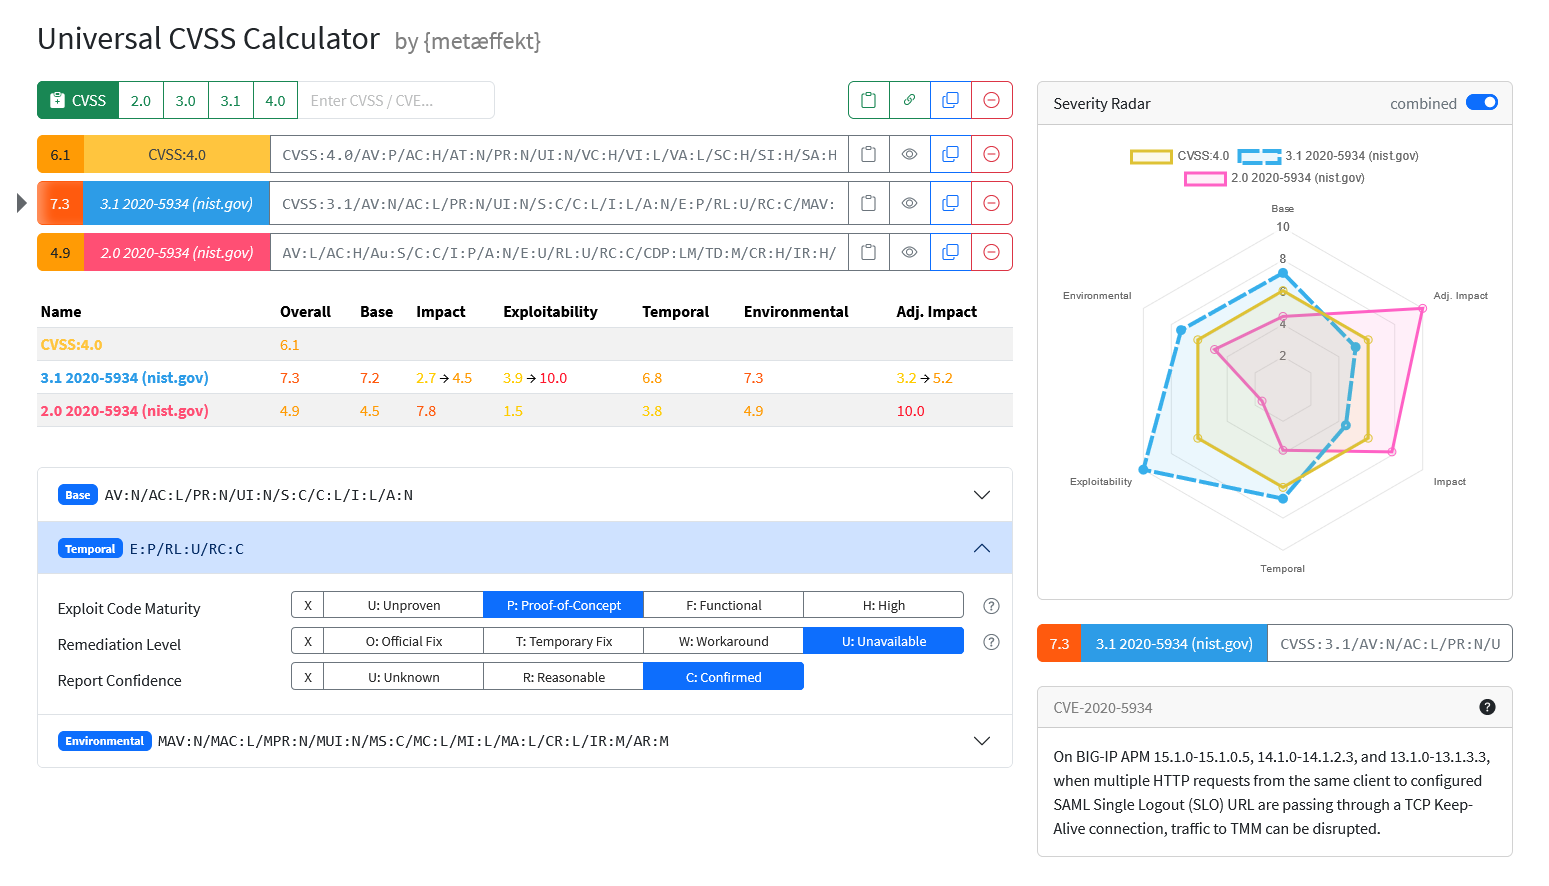
\includegraphics[width=0.8\textwidth, keepaspectratio]{res/img/metaeffekt-cvss-calculator-ui}
    \caption{Der {\metaeffekt} Universal CVSS-Rechner}
    \label{fig:metaeffekt-cvss-calculator-ui}
\end{figure}

Von Herrn Shane Coughlan (OpenChain General Manager und ein Referent vom Open Source Forum der bitkom) haben wir freundlicherweise folgendes Zitat zu unserem Rechner erhalten:
\begin{quote}
    \textit{\qt{Contextualizing security threats is as important as identifying their existence,” says Shane Coughlan, OpenChain General Manager. “The emergence of open source tools to visualize this is a key part of ensuring the supply chain can plan ahead and action responses. We are delighted to see the work by Metaeffekt, an official OpenChain Partner, in the domain. It aligns well with OpenChain ISO/IEC 18974, the international standard for open source security assurance.}}
\end{quote}
